\section{Evaluation}
The goal of this evaluation is to investigate the applicability of the proposed matrix-based algorithm to CFPQ with all-path query semantics and to provide the comparation of the most performant linear algebra-based CFPQ algorithms. We will compare the following CFPQ implementations:
\begin{itemize}
	\item $MtxSingle$ --- the implementation from~\cite{10.1145/3398682.3399163} of the matrix-based CFPQ algorithm for the single-path query semantics,
	\item $Tns$ --- the implementation from~\cite{kron} of the Kronecker product-based CFPQ algorithm for all three query semantics including the all-path query semantics,
	\item $MtxAll$ --- the implementation of the proposed matrix-based CFPQ algorithm for all-path query semantics which utilizes SuiteSparse\footnote{SuiteSparse is a sparse matrix software which includes GraphBLAS API implementation. Project web page: \url{http://faculty.cse.tamu.edu/davis/suitesparse.html}. Access date: 14.01.2021.}~\cite{Davis2018Algorithm9S} implementation of GraphBLAS API for matrix manipulations.
\end{itemize}

All implementations utilize CPU and represent matrices in sparse format. First, we measured the execution time and required memory of the index creation. Then we compared the practical applicability of the paths extraction for both implementations $MtxAll$ and $Tns$ of the CFPQ with all-path query semantics.

For evaluation, we used a PC with Ubuntu 18.04 installed.
It has Intel core i7-6700 CPU, 3.4GHz, and DDR4 64Gb RAM.
We only measure the execution time of the algorithms themselves, thus we assume an input graph is loaded into RAM in the form of its adjacency matrix in the sparse format.

\subsection{Dataset Description}

We use the graphs and respective queries from the CFPQ\_Data dataset\footnote{CFPQ\_Data dataset GitHub repository: \url{https://github.com/JetBrains-Research/CFPQ_Data}. Access date: 14.01.2021.} provided in~\cite{10.1145/3398682.3399163} that contains the real-world RDFs with properties presented in table~\ref{tbl:propRDF}, and queries $g_1, g_2, geo$ 
that are variations of the \textit{same-generation query}~\cite{FndDB} --- an important example of real-world queries that are context-free but not regular.




{\setlength{\tabcolsep}{0.25em}
	\begin{table}
		{
			\caption{RDFs properties}
			\label{tbl:propRDF}
			\small
			\rowcolors{2}{black!2}{black!10}
			\begin{tabular}{|l|c|c|c|}
				\hline
				Graph & \#V & \#E & Queries \\
				\hline
				\hline
				pathways               & 6238                 & 18 598               & $g_1, g_2$ \\
				gohierarchy            & 45 007               & 980 218              & $g_1, g_2$ \\
				enzyme                 & 48 815               & 109 695              & $g_1, g_2$ \\
				eclass\_514en          & 239 111              & 523 727              & $g_1, g_2$ \\
				go                     & 272 770              & 534 311              & $g_1, g_2$ \\
				geospecies             & 450 609              & 2 311 461            & $g_1, g_2, geo$  \\
				taxonomy                   & 5 728 398                 & 14 922 125                 & $g_1, g_2$ \\
				\hline
			\end{tabular}
		}
	\end{table}
}


\subsection{Evaluation Results}
The results of the index creation for all three implementations are presented in Table~\ref{tbl:index_creation}. We can see that the running time of all implementations is
small in almost all cases. The most performant implementation is $MtxSingle$ especially on big graphs. Weaker single-path query semantics is the reason for such results since we can use more simple index to restore only one path per vertex pair. However, the Kronecker product-based implementation $Tns$ uses more complex but compact index and consumes less memory. The implementation $MtxAll$ of the proposed matrix-based CFPQ algorithm for all-path query semantics has comparable to $Tns$ execution time on small graphs but significantly bigger execution time on big graphs with complex structure. Also, the $MtxAll$ 
consumes significantly more memory than $Tns$. The reason of such behavior is that the proposed matrix-based algorithm is trying to store the information of all founded paths more explicitly. Also, the index constructed by $MtxAll$ is less compact than one constructed by $Tns$. On the biggest $taxonomy$ graph and query $g_1$ we even have the out of memory error for $MtxAll$ implementation.

After constructing the index, we compared the execution time of the path extraction for CFPQ with all-path query semantics using both $MtxAll$ and $Tns$ implementations. The results of path extraction are presented in Figures~\ref{fig:extractTimeTns} and \ref{fig:extractTimeMtx} (boxplots are standard, medians are indicated and outliers are omitted). For computation termination, we limit maximum paths length to 10. After that we extract paths for each vertex pair and group the execution time of the path extraction algorithms by the number of paths returned. We can see that the path extraction running time of the implementation $MtxAll$ of the proposed matrix-based algorithm is up to 1000 times faster than for the Kronecker product-based implementation $Tns$. As was mentioned above, in the proposed matrix-based CFPQ algorithm we construct an index with more explicit information about all founded paths. Thus, such paths can be restored significantly faster than using the Kronecker product-based algorithm.

We can conclude, that the proposed matrix-based CFPQ algorithm for all-path query semantics is still performant enough for real-world data analysis. Also, we can conclude the following.

\begin{itemize}
	\item As shown in~\cite{10.1145/3398682.3399163, kron} the most performant algorithm for the CFPQ with relational query semantics when the paths extraction is not required is the Azimov's matrix-based algorithm from~\cite{Azimov:2018:CPQ:3210259.3210264}.
	\item For single-path query semantics when only one path per each vertex pair is required, the Azimov's matrix-based CFPQ algorithm~\cite{10.1145/3398682.3399163} for single-path query semantics is most performant.
	\item For all-path query semantics, the proposed matrix-based and the Kronecker product-based CFPQ algorithms have the following tradeoffs. If it is necessary  to frequently recalculate the index for a changing graph or a path query then the best choice is the Kronecker product-based algorithm~\cite{kron} with faster and less memory consuming index construction. If it is necessary to extract paths many times for one constructed index then the proposed matrix-based CFPQ algorithm is preferable.
\end{itemize}

{\setlength{\tabcolsep}{0.25em}
	\begin{table*}[t]
		{
			\caption{Index creation time in seconds and memory in megabytes where we use "---" to indicate that the query is not applicable to the graph and we use "$err$" in case of out of memory error }
			\label{tbl:index_creation}
			\small
			\rowcolors{4}{black!2}{black!10}
			\begin{tabular}{|l|l|l|l|l|l|l|l|l|l|l|l|l|l|l|l|l|l|l|}
				\hline
				\multicolumn{1}{|c|}{\multirow{3}{*}{Graph}} & \multicolumn{6}{c|}{G1}                                                           & \multicolumn{6}{c|}{G2}                                                           & \multicolumn{6}{c|}{Geo}                                                          \\ \cline{2-19}
				\multicolumn{1}{|c|}{}                       & \multicolumn{2}{c|}{MtxAll} & \multicolumn{2}{c|}{Tns} & \multicolumn{2}{c|}{MtxSingle} & \multicolumn{2}{c|}{MtxAll} & \multicolumn{2}{c|}{Tns} & \multicolumn{2}{c|}{MtxSingle} & \multicolumn{2}{c|}{MtxAll} & \multicolumn{2}{c|}{Tns} & \multicolumn{2}{c|}{MtxSingle} \\ \cline{2-19}
				\multicolumn{1}{|c|}{}                       & Time          & Mem         & Time        & Mem        & Time        & Mem        & Time          & Mem         & Time        & Mem        & Time        & Mem        & Time          & Mem         & Time        & Mem        & Time        & Mem        \\ \hline \hline
				pathways                                     & 0.04          & 91          & 0.02        & 123        & 0.01        & 671        & 0.01          & 49          & 0.01        & 122        & 0.01        & 671        & ---           & ---         & ---         & ---        & ---         & ---        \\ \hline
				go-hierarchy                                 & 22.12         & 38797       & 0.17        & 265        & 1.41        & 660        & 15.66         & 28447       & 0.24        & 252        & 0.84        & 671        & ---           & ---         & ---         & ---        & ---         & ---        \\ \hline
				enzyme                                       & 0.4           & 307         & 0.04        & 137        & 0.01        & 216        & 0.02          & 61          & 0.02        & 132        & 0.01        & 217        & ---           & ---         & ---         & ---        & ---         & ---        \\ \hline
				eclass\_514en                                & 25.02         & 14416       & 0.24        & 205        & 0.23        & 216        & 0.22          & 126         & 0.27        & 193        & 0.16        & 216        & ---           & ---         & ---         & ---        & ---         & ---        \\ \hline
				go                                           & 11.8          & 8290        & 1.58        & 282        & 1.45        & 215        & 1.13          & 990         & 1.27        & 243        & 0.93        & 217        & ---           & ---         & ---         & ---        & ---         & ---        \\ \hline
				geospecies                                   & 4.45          & 2691        & 0.08        & 218        & 0.06        & 2250       & 0.34          & 156         & 0.01        & 196        & 0.01        & 2251       & 32.06         & 44235       & 26.32       & 19537      & 15.54       & 22941      \\ \hline
				taxonomy                                     & $err$           & $err$         & 4.42        & 2018       & 2.73        & 1962       & 19.13         & 27232       & 3.56        & 1776       & 1.15        & 2250       & ---           & ---         & ---         & ---        & ---         & ---        \\ \hline
			\end{tabular}
		}
	\end{table*}
}

\begin{figure*}
	\begin{subfigure}{0.32\textwidth}
		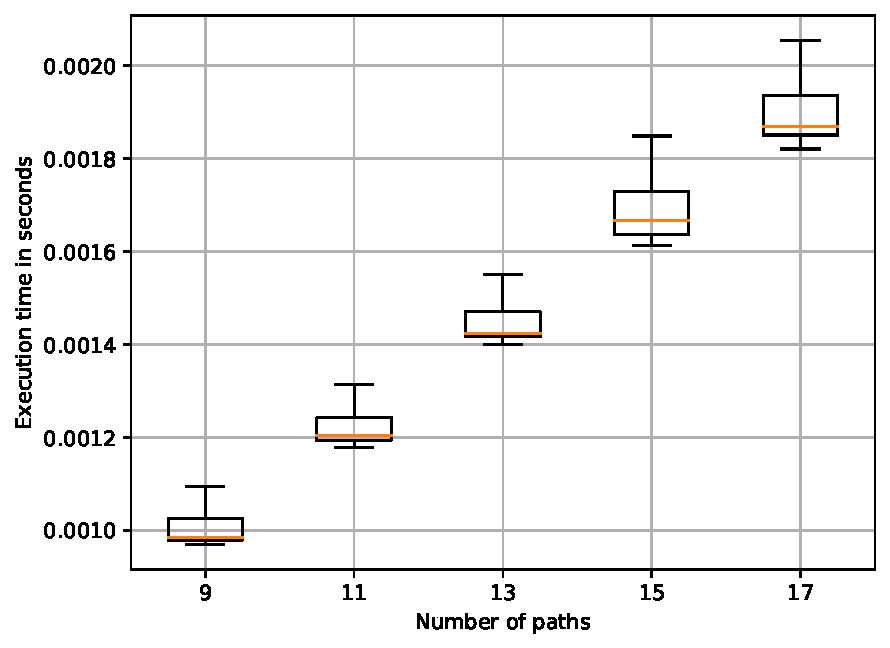
\includegraphics[width=\linewidth,trim=0 0 -1.5cm 0]{pictures/tensor_eclass_514en_10_small.pdf}
		\caption{$eclass\_514en$ and $g_1$} \label{fig:extractTimeEclassTns}
	\end{subfigure}
	\hspace*{\fill} % separation between the subfigures
	\begin{subfigure}{0.32\textwidth}
		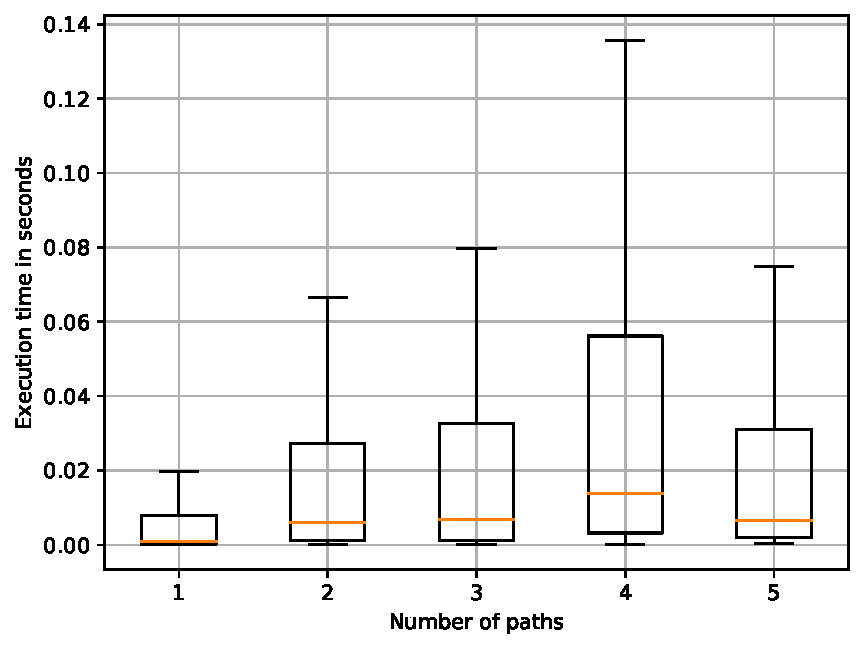
\includegraphics[width=\linewidth,trim=0 0 -1.5cm 0]{pictures/tensor_go_10_small.pdf}
		\caption{$go$ and $g_1$ for small number of paths} \label{fig:extractTimeGoSmallTns}
	\end{subfigure}
	\hspace*{\fill} % separation between the subfigures
	\begin{subfigure}{0.32\textwidth}
		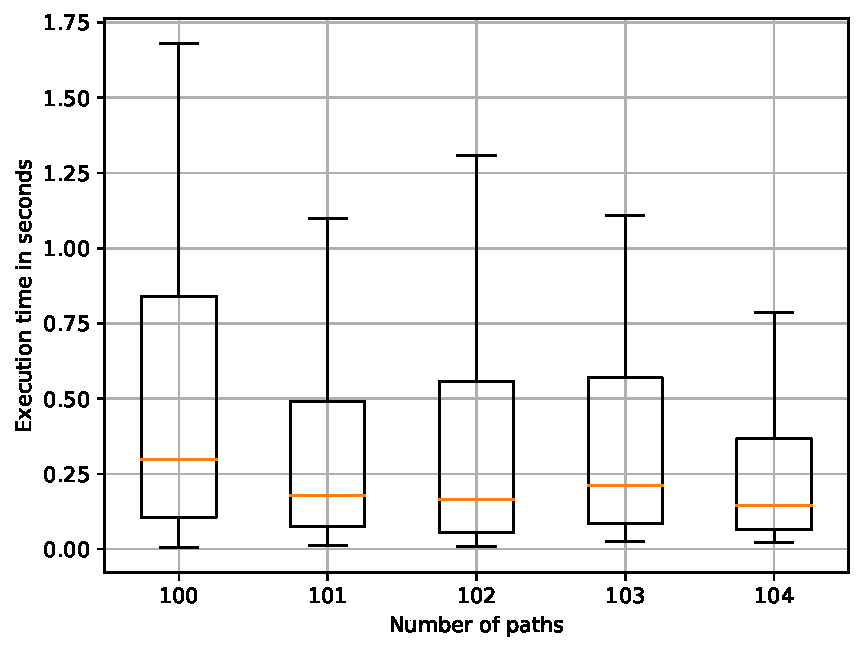
\includegraphics[width=\linewidth,trim=0 0 -1.5cm 0]{pictures/tensor_go_10_big.pdf}
		\caption{$go$ and $g_1$ for big number of paths} \label{fig:extractTimeGoBigTns}
	\end{subfigure}
	\caption{Execution time of the Kronecker product-based path extraction algorithm from~\cite{kron} implemented in $Tns$ depending on the number of paths returned}
	\label{fig:extractTimeTns}
\end{figure*}

\begin{figure*}
	\begin{subfigure}{0.32\textwidth}
		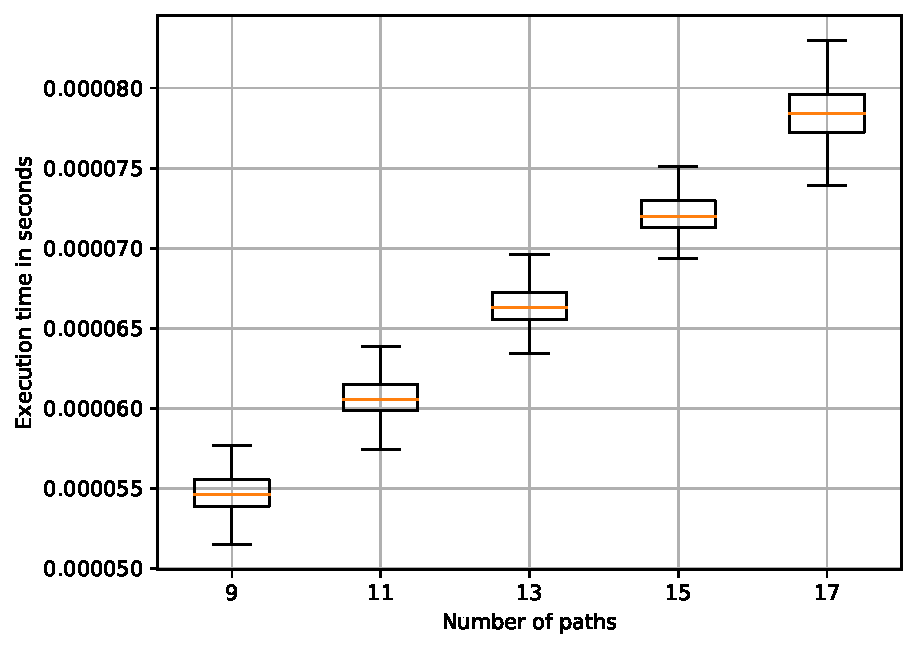
\includegraphics[width=\linewidth,trim=0 0 -1.5cm 0]{pictures/allMatr_eclass_514en_10_small.pdf}
		\caption{$eclass\_514en$ and $g_1$} \label{fig:extractTimeEclassMtx}
	\end{subfigure}
	\hspace*{\fill} % separation between the subfigures
	\begin{subfigure}{0.32\textwidth}
		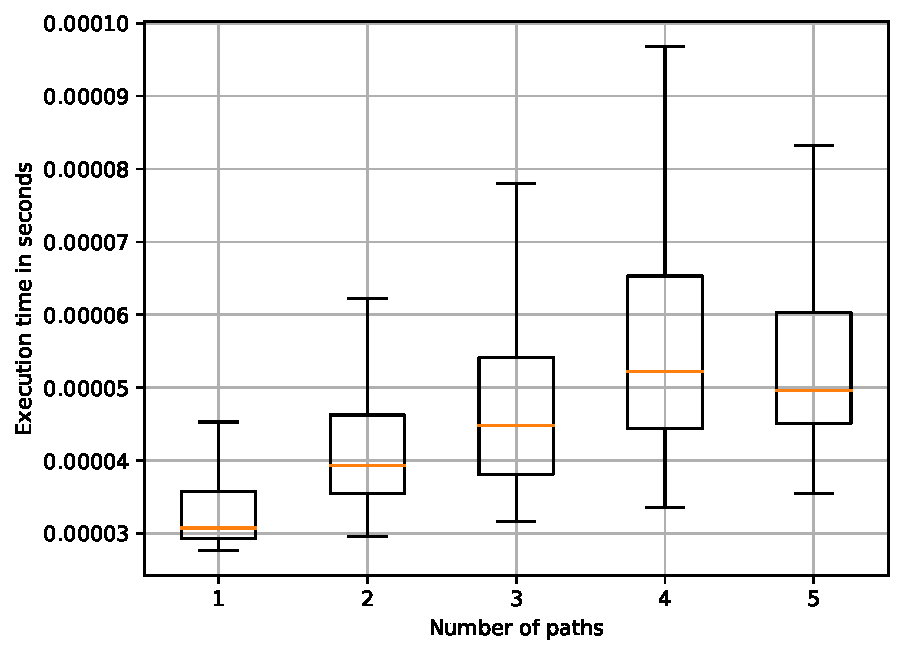
\includegraphics[width=\linewidth,trim=0 0 -1.5cm 0]{pictures/allMatr_go_10_small.pdf}
		\caption{$go$ and $g_1$ for small number of paths} \label{fig:extractTimeGoSmallMtx}
	\end{subfigure}
	\hspace*{\fill} % separation between the subfigures
	\begin{subfigure}{0.32\textwidth}
		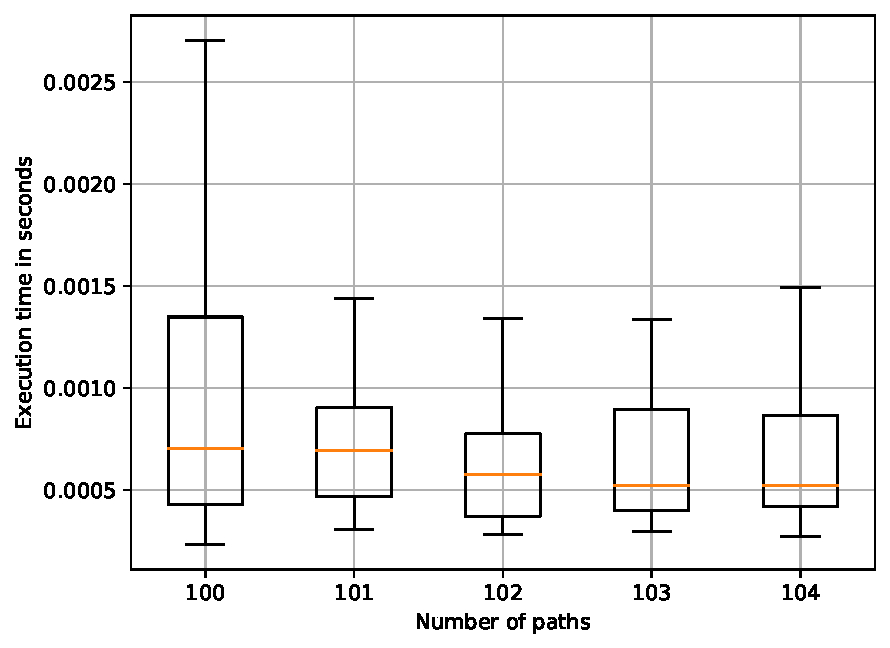
\includegraphics[width=\linewidth,trim=0 0 -1.5cm 0]{pictures/allMatr_go_10_big.pdf}
		\caption{$go$ and $g_1$ for big number of paths} \label{fig:extractTimeGoBigMtx}
	\end{subfigure}
	\caption{Execution time of the proposed matrix-based path extraction algorithm implemented in $MtxAll$ depending on the number of paths returned}
	\label{fig:extractTimeMtx}
\end{figure*}
